\documentclass[10pt,a4paper]{article}

\usepackage{graphicx}    
\usepackage{float}
\usepackage{hyperref}                   % collegamenti ipertestuali
\usepackage[utf8]{inputenc}
\usepackage[english]{babel}
\usepackage[babel]{csquotes}
\usepackage{url}
\usepackage{graphicx}
\usepackage{lastpage}
\usepackage{fancyhdr}
\usepackage[top=1cm,bottom=4cm,left=80pt,right=80pt]{geometry} %disegna la linea
\usepackage{listings} %per grandi porzioni di codice
\usepackage{booktabs,tabularx}
\usepackage{makeidx}
\usepackage{fixltx2e}
\usepackage{hyperref}
\usepackage{enumitem}
\usepackage{color}
\usepackage[T1]{fontenc}
\usepackage{svg}
\usepackage{amsmath}
\usepackage[toc]{glossaries}
\usepackage{dirtree}
\usepackage{listings}
\usepackage{siunitx}
\usepackage[official]{eurosym}
\usepackage[export]{adjustbox}
\usepackage{calc}
\usepackage{rotating}
\usepackage{soul}
\usepackage{amsmath}

\pagestyle{fancy}
\setlength{\headheight}{2cm} %settato grandezza header

\renewcommand{\footrulewidth}{0.5pt} %ridefinisco il valore della riga di intestazione
\renewcommand{\headrulewidth}{0.5pt} %ridefinisco il valore della riga di pie' di pagina
\addtolength{\headwidth}{\marginparsep}
\addtolength{\headwidth}{\marginparwidth}

\fancyhead{} %annulla head di default
\fancyfoot{} %annulla foot di default


\newcommand{\complex}[1]{\textit{\color{blue} {#1}}}
\newcommand{\change}[1]{\textit{ \color{red}** {#1}}}

%%%%%%%%%%%%%%%%%%%%%%%%%%%%%%%%%%%%%%%%%%%%%%%%%%%%%%%%%%%%%%%%%%%%%
%    DOCUMENT TITLE

\newcommand{\doctitle}{\textbf{CondorcetFuse} \\
	 Condoret voting for run fusion}

%%%%%%%%%%%%%%%%%%%%%%%%%%%%%%%%%%%%%%%%%%%%%%%%%%%%%%%%%%%%%%%%%%%%%
%%%%%%%%%%%%%%%%%%%%%%%%%%%%%%%%%%%%%%%%%%%%%%%%%%%%%%%%%%%%%%%%%%%%%
%%%%%%%%%%%%%%%%%%%%%%%%%%%%%%%%%%%%%%%%%%%%%%%%%%%%%%%%%%%%%%%%%%%%%
%   DOCUMENT SUBTITILE
\newcommand{\docsubtitle}{Evalutation and comparison of an implementation with other fusion strategies}
%%%%%%%%%%%%%%%%%%%%%%%%%%%%%%%%%%%%%%%%%%%%%%%%%%%%%%%%%%%%%%%%%%%%%
%%%%%%%%%%%%%%%%%%%%%%%%%%%%%%%%%%%%%%%%%%%%%%%%%%%%%%%%%%%%%%%%%%%%%
%%%%%%%%%%%%%%%%%%%%%%%%%%%%%%%%%%%%%%%%%%%%%%%%%%%%%%%%%%%%%%%%%%%%%
%   DOCUMENT FOOTER 
% If not modified, footer is equal to document subtitle
\newcommand{\projectfooter}{\docsubtitle}
%%%%%%%%%%%%%%%%%%%%%%%%%%%%%%%%%%%%%%%%%%%%%%%%%%%%%%%%%%%%%%%%%%%%%
%%%%%%%%%%%%%%%%%%%%%%%%%%%%%%%%%%%%%%%%%%%%%%%%%%%%%%%%%%%%%%%%%%%%%
%%%%%%%%%%%%%%%%%%%%%%%%%%%%%%%%%%%%%%%%%%%%%%%%%%%%%%%%%%%%%%%%%%%%%


%	Logo intestazione
%\rhead{\includegraphics[scale=0.15]{}}

%	footer
\cfoot{
	\projectfooter\\
	{\doctitle}\\
}
\rfoot{
	\thepage\ di \pageref{LastPage}
}


%**************************************************************
% Impostazioni di hyperref
%**************************************************************
\hypersetup{
	%hyperfootnotes=false,
	%pdfpagelabels,
	%draft,	% = elimina tutti i link (utile per stampe in bianco e nero)
	colorlinks=true,
	linktocpage=true,
	pdfstartpage=1,
	pdfstartview=FitV,
	% decommenta la riga seguente per avere link in nero (per esempio per la stampa in bianco e nero)
	%colorlinks=false, linktocpage=false, pdfborder={0 0 0}, pdfstartpage=1, pdfstartview=FitV,
	breaklinks=true,
	pdfpagemode=UseNone,
	pageanchor=true,
	pdfpagemode=UseOutlines,
	plainpages=false,
	bookmarksnumbered,
	bookmarksopen=true,
	bookmarksopenlevel=1,
	hypertexnames=true,
	pdfhighlight=/O
}
\newcommand{\printTitle}{	
	\begin{titlepage}
		\begin{center}
			
		%	\begin{figure}[h!]	\vspace{5cm}
		%		\centering
		%		\includegraphics[width=0.7\linewidth]{}
		%	\end{figure}
			\vspace{0.3cm}
			\hrule
			\vspace{0.3cm}	
			\begin{Huge}
				\doctitle  \\			
			\end{Huge}
			\vspace{0.3cm}
			\begin{Large}
				\docsubtitle
			\end{Large}
			\vspace{0.3cm}
			
		\end{center}
		
\end{titlepage}}






\begin{document}
    \printTitle
    \newpage
    \tableofcontents
    \newpage
    %\listoftables
    %\listoffigures

    \section{Introduction}
      Fusion in information retrieval is combination of retrieval results computed with multiple different retrieval systems into one single ``fused'' result. This process aim to improve basic systems performances. 
   
   Some previous results show that this technique  can greatly improve retrieval
   effectiveness over that of the individual results.
   
   The aim of this work is to present a possible implementation of some basic
   fusion strategies and compare them to an advanced one: Condorcet fusion \cite{3}.
   
   In this project the input documents were taken from the TREC TIPSTER Collection using 50 topics (topics 351-400).
   We used Terrier for retrieval and indexing and MATTERS for evaluation.
   
   We organized our work as follows:

    \begin{itemize}
        \item \textbf{Indexing:} we created four different indexes:
        \begin{itemize}
        	\item Without both stemmer and stop list;
        	\item only using the Porter stemmer;
        	\item only using the stop list;
        	\item using both the Porter stemmer and the stop list;
        \end{itemize}
        \item \textbf{Retrieval:} 10 different retrieval models listed in Table \ref{tab:10Mod};
		\item \textbf{Normalization:} min/max normalization as presented by Lee \cite{1}
        \item \textbf{Fusion strategy:} we compared seven different fusion strategies:
            \begin{itemize}
                \item 6 basic strategies proposed by Fox and Shawn \cite{2} and listed in Table \ref{tab:6Fus};
                \item Condorcet fusion (advanced strategy) as proposed by Montague and Aslam \cite{3}
            \end{itemize}
    \end{itemize}

	\begin{table} [H]
		\begin{minipage} {0.2\linewidth}
			\centering
			\begin{tabular}{l}
				\toprule
				\textbf{Retrieval models} \\ \toprule
				BB2 \\
				BM25 \\
				DLH13 \\
				Hiemstra\_LM \\
				IFB2 \\
				TF\_IDF \\
				DFIC \\
				DFIZ \\
				DirichletLM \\
				InL2 \\
				\bottomrule
			\end{tabular}
			\caption{Retrieval models used}
			\label{tab:10Mod}
		\end{minipage}		
		\begin{minipage} {0.8\linewidth}
			\centering
			{\def\arraystretch{2}\tabcolsep=10pt
			\begin{tabular}{l p{5cm}}
				\toprule
				\textbf{Basic fusion methods} & \textbf{New score formula} \\ \toprule
				CombMNZ & $(\sum_{i}^{N} s_{i})*(Num~s_{i}\ne 0)$ \\ \hline
				CombSUM & $ \sum_{i}^{N} s_{i} $ \\ \hline
				CombMIN & $ min_{i}^{N} {(s_{i})} $ \\ \hline
				CombMAX & $ max_{i}^{N} {(s_{i})} $  \\ \hline
				CombMED & $ median_{i}^{N} {(s_{i})} $ \\ \hline
				CombANZ & $  (\sum_{i}^{N} s_{i}) /
							(Num ~ s_{i} \ne 0)$   \\ 
							\bottomrule
			\end{tabular}}
			\caption{Basic fusion methods used }
			\label{tab:6Fus}
		\end{minipage}		
	\end{table}
    
  \section{Condorcet Fusion}
% The Condorcet Fusion strategy considers the ranking of documents from different systems as an instance of the voting problem where documents are candidates and each input retrieval system is a voter.

Condorcet-fuse strategy merges single systems results considering the document ranking problem like a voting problem between different systems. 


The output of each input system is seen as a list of preferences, where the higher ranked documents beat the lower ranked ones.

The result of Condorcet Fusion is computed like a majoritarian voting between each system preference for each document-query pair. 
A system preference is its output ranking list for a given query.  


Having the lists of different preferences, Condorcet-fuse orders the documents using the Condorcet voting algorithm, estimating the final ordering for a given document-query pair considering the most voted 
voted rank between systems' preferences on that pair. 


\subsection{The Condorcet Graph}

A Condorcet Graph can be used to represent the majoritarian preference for each document on a given query. 

Given 10 models of retrieval with n documents, the corresponding
Condorcet graph $G = (V, E)$ has one vertex for each of the n documents.

For each document pair (x, y), there exists an edge from x to
y (denoted by $x \rightarrow y$) if x would receive at least as many votes as y in a head-to-head contest.

Cycles can simply be viewed as ties.
Montague and Aslam \cite{3} suggest a Condorcet fusion implementation that allow graph nodes ordering in a efficient manner (time $O(n*\log(n))$) .  

\section{Implementation}

We follow the Condorcet Fuse implementation suggested by Montague and Aslam \cite{3}.

We choose to assign some dummy relevance score to Condorcet's output, the score is assigned based on the rank.

The implementation of Condorcet uses Quicksort, with the following algorithm
as comparing function:

\hfill
\begin{lstlisting}
	count = 0
	for each of the k search systems do:

		if (sys_i ranks d1 above d2)  count = count+1 
		if (sys_i ranks d2 above d1)  count = count-1 

		if (count > 0)  rank d1 better than d2
		else  rank d2 better than d2 
		
\end{lstlisting}
\hfill
\\
For more information on the code, see \href{https://github.com/annabonaldo/IRCondorcetFuse/blob/master/README.md}{README} in our {\href{https://github.com/annabonaldo/IRCondorcetFuse}{code repository }
    \section{Evaluation}
    % Modelli scelti 
    % Indicizzazione utilizzata

	The evaluation criteria based on the given \textbf{pool uses a binary relevance score}:
	Relevant and Non-Relevant.
	The documents left out from the pool are considered to be Non-Relevant.
	We decided to use \textbf{Average Precision} to evaluate a run on the set of topics and \textbf{Mean Average Precision} to evaluate a run between different retrieval systems. We always work on normalized data.
	
	We first did an analysis considering the 10 models presented in Table \ref{tab:10Mod} running retrieval and indexing with Terrier's default settings (that is, using both the Porter Stemmer and a stop list) and the fusion's given these 10 input systems.
	
	Then, since the paper on Condorcet Fuse performed some analysis to understand the relation between CondFuse's MAP and the number of input systems, we also tried something similar. 
	
	\subsection{First Analysis}
	At first, we wanted to see if using a fusion strategy actually improves the best performance of a simple model run with both the stemmer (we used Porter Stemmer) and a stop list.
	We proceeded as follows:
	\begin{enumerate}
		\item We computed the AP and the MAP for the 10 input models;
		\item We computed the AP and the MAP for the 7 fusion models (6 basic and Condorcet);
		\item We selected the 5 systems with the best MAP values.
	\end{enumerate}
	Figure \ref{fig:top5AP} shows the Average Precision for the top 5 best systems, while Table \hyperref[tab:17SysMAP]{3} shows the MAP for all of them.
	
	\begin{figure}[H]
		\begin{minipage}{0.7\textwidth}				
			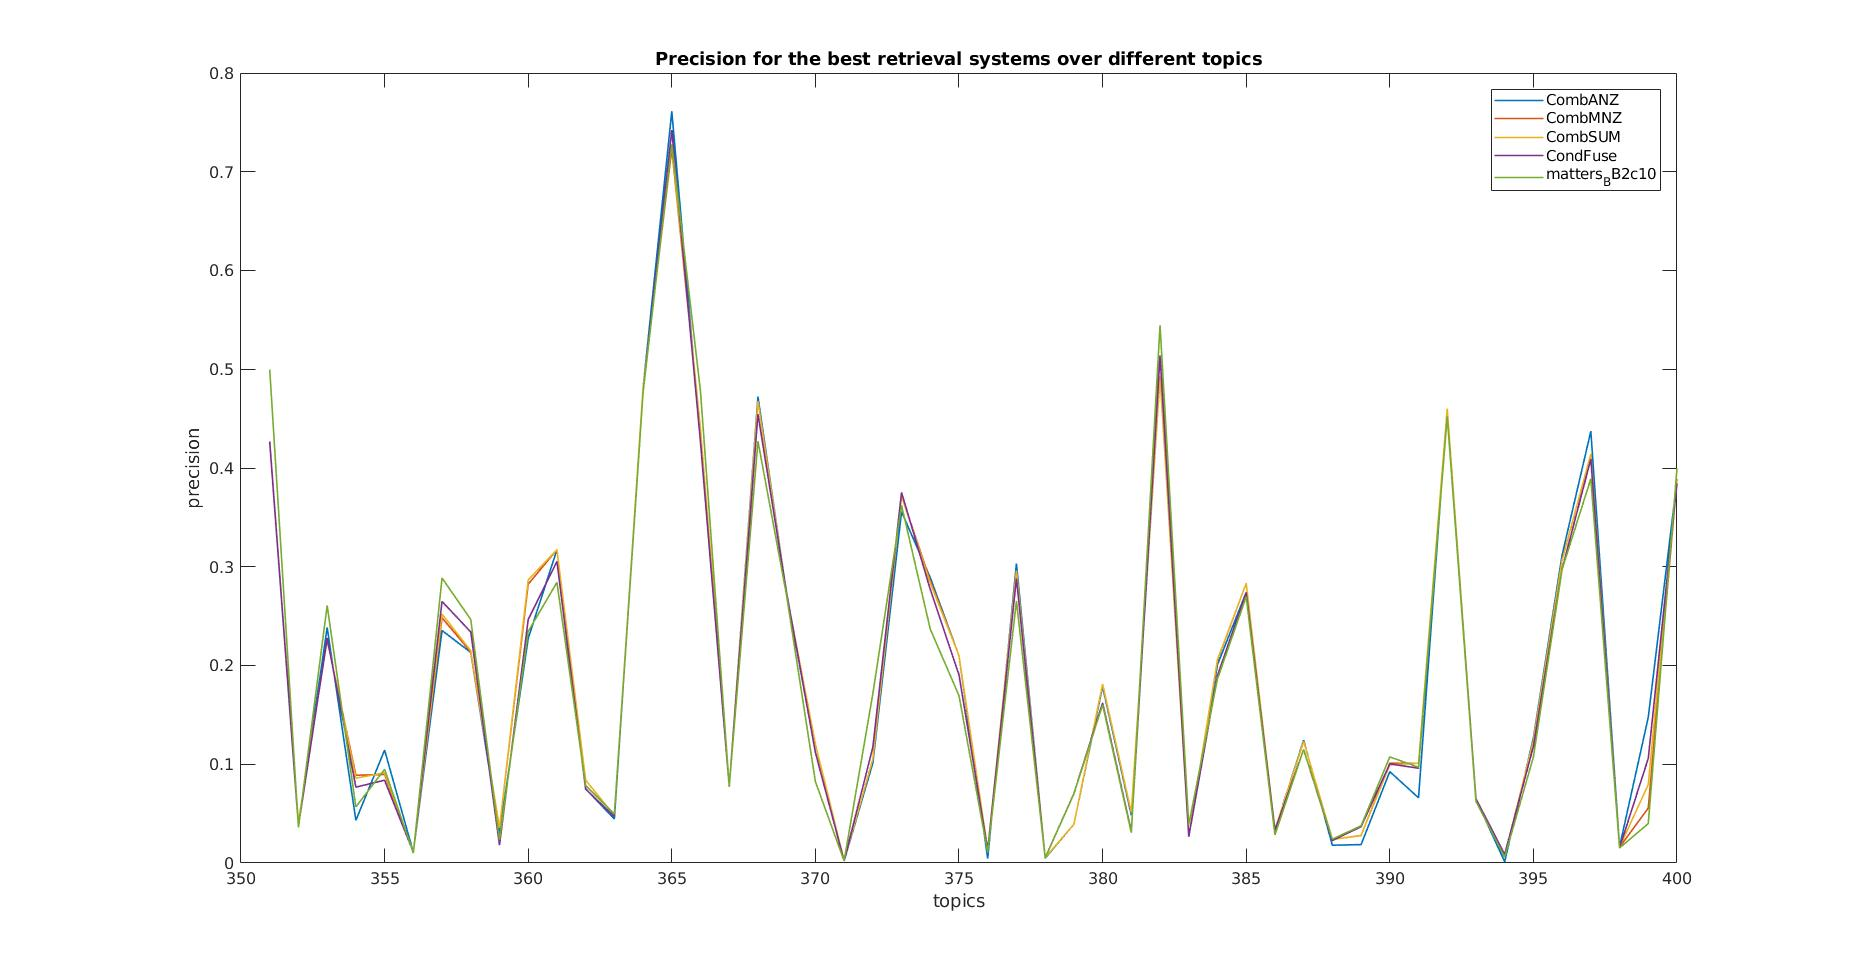
\includegraphics[width=\linewidth]{../eval/results-img-graphs/top5.jpg}
			\caption{AP over 50 topics for the 5 best systems}
			\label{fig:top5AP}
		\end{minipage}
		\begin{minipage}{0.3\textwidth}
			\begin{tabular}{c c}
					\toprule
					\textbf{Systems} & \textbf{MAP}\\ \toprule
					CombSUM & 0.1909 \\
					CombMNZ & 0.1902 \\
					CombANZ & 0.1891 \\
					CondFuse & 0.1883 \\
					BB2 & 0.1881 \\
					IFB2 & 0.1880 \\					
					DirichletLM & 0.1862 \\
					InL2 & 0.1853 \\
					CombMED & 0.1840 \\
					DLH13 & 0.1829 \\				
					BM25 & 0.1827 \\
					TF\_IDF & 0.1821\\
					CombMAX & 0.1817 \\
					DFIZ & 0.1783 \\					
					DFIC & 0.1758 \\				
					Hiemstra\_LM & 0.1733 \\
					CombMIN & 0.1515 \\							
					\bottomrule
				\end{tabular}
			\captionof {Table 3: }{Retrieval systems sorted by decreasing MAP}
			\label{tab:17SysMAP}
		\end{minipage}			
	\end{figure}

	\subsubsection{Results Analysis}
	The results of these first tests show that it is generally convenient to use a fusion method.
	Four out of the top five best systems where fusion systems, with Condorcet Fuse being the fourth best overall.
	
	But, we also noted that the performances of the methods are all very close, and the best and worse topics are the same regardless of the system used.
	
	\subsection{Further Analysis}
	We decided we wanted to test how the performances of the 10 input systems affected the performance of the fusion methods.
	Furthermore, since Montague and Aslam \cite{3} analyzed the algorithm's performance over the number of input systems, we also tried fusions starting with 2 input systems up to 10.
	
	\subsubsection{Analysis over increasing number of inputs}	
	Figure \ref{fig:4x4comp} shows a comparison between the MAP for the 7 fusion methods over the number of input systems and with different indexing and retrieval settings.
	
	\begin{figure}[h]
		\centering				
		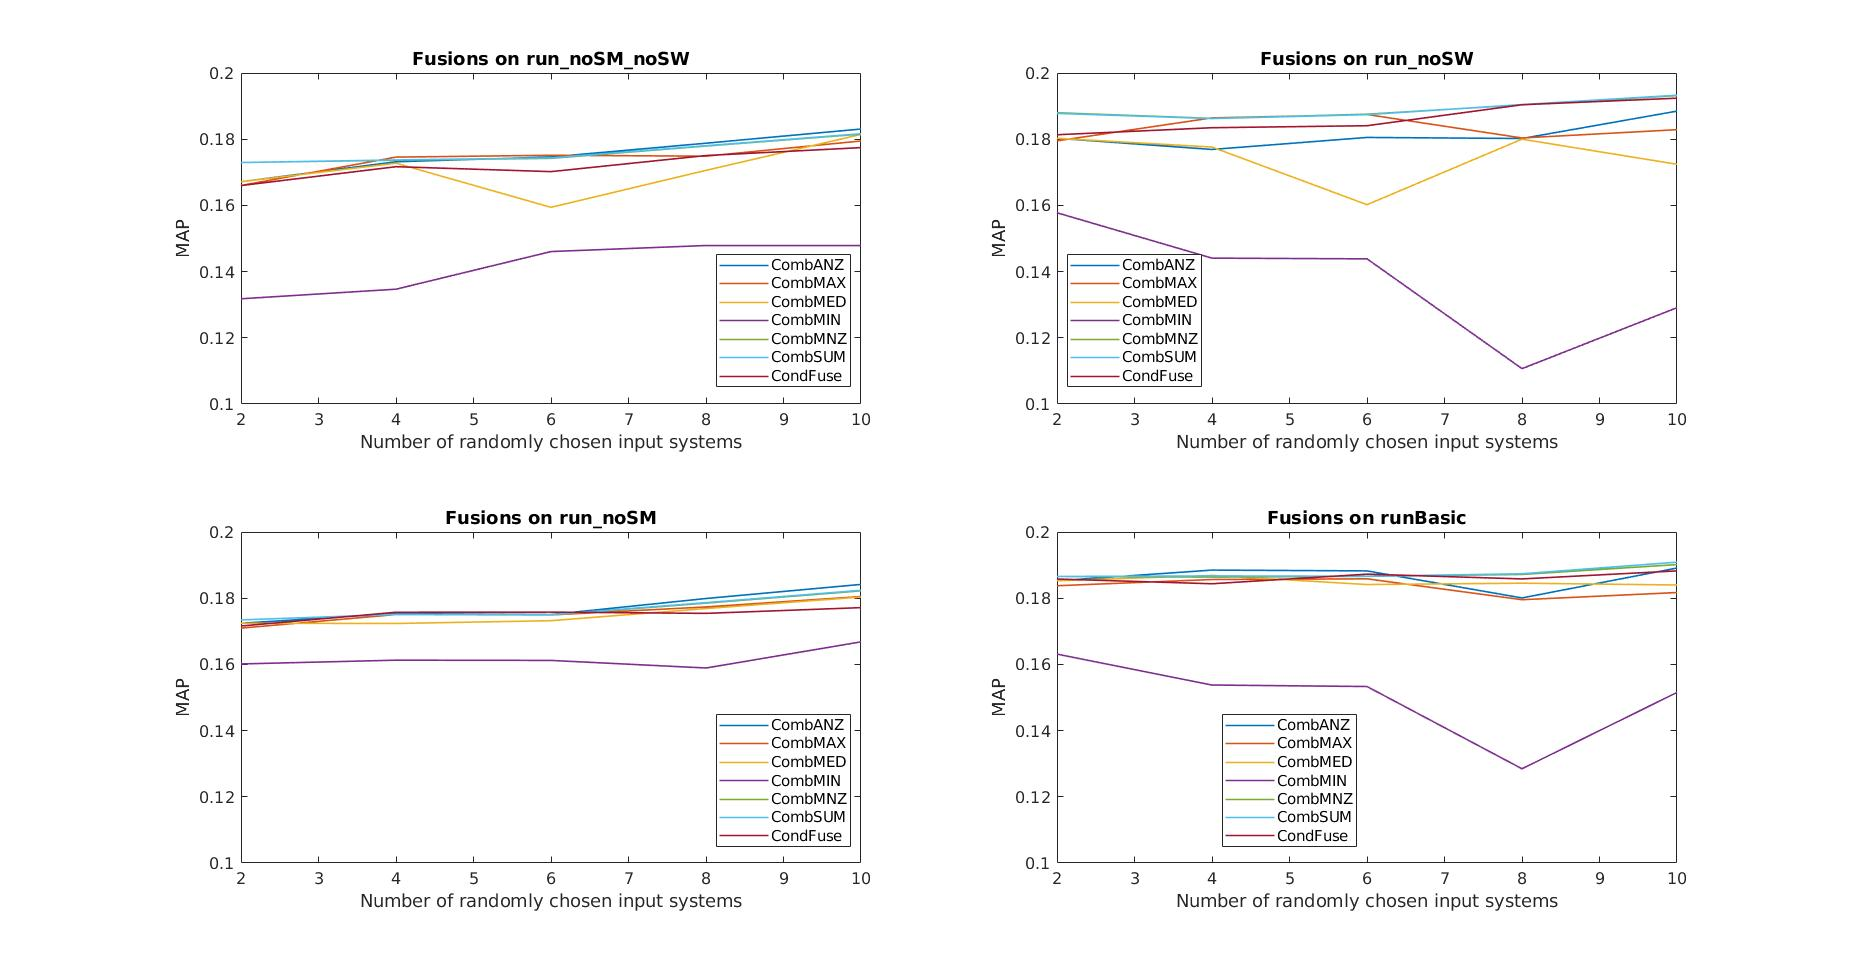
\includegraphics[width=\linewidth]{../eval/results-img-graphs/4x4comp.jpg}
		\caption{MAP depending in the number of input system and indexing and retrieval settings}				
		\label{fig:4x4comp}					
	\end{figure}

	We noted that the number of input system doesn't much affect the performances of the fusion methods. The main difference was given by the indexing and retrieval settings. In particular, having neither the stemmer or the stoplist was similar to having just the stop list, while having both stemmer and stoplist was more similar to just having the stemmer.
	
	We expected the stop list to be more defining than the stemmer, so we performed some further analysis focusing on what affected more the fusions.
	
	\subsubsection{Analysis on the indexing and retrieval settings}
	We wanted to see how the indexing and retrieval settings affect the fusions' performances. Furthermore, we wanted to understand the relationship between the models' and the fusions' performances.
	We chose to focus on the fusions performed over 10 input systems. 
	
	Figure \ref{fig:MAPMod} shows the MAP's values for the 10 models over different indexing and retrieval settings, while Figure \ref{fig:MAPFus} shows the performance of the fusion  method of over the same 10 models with the same settings. CombMIN is not in the graph because of its poor performances and to have a better comparison between the 2 Figures.
	
	\begin{figure}[H]
		\begin{minipage}{0.5\linewidth}
			\centering
			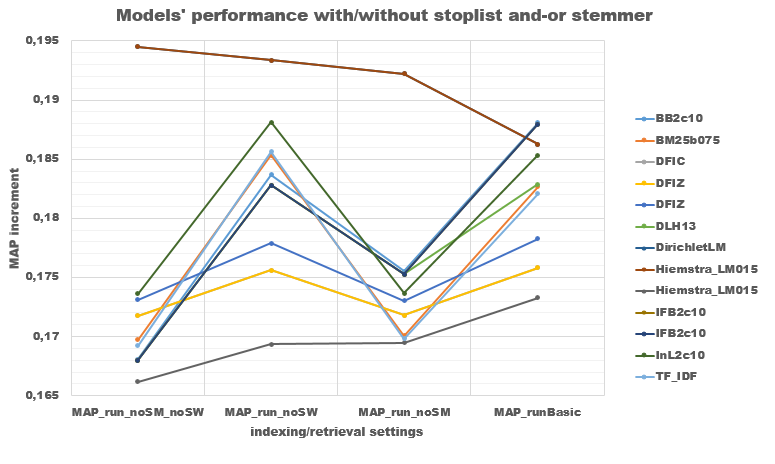
\includegraphics[width=\linewidth]{../eval/results-img-graphs/MAPModSMSW.png}
			\caption{MAP for the retrieval models over different indexing and retrieval settings}				
			\label{fig:MAPMod}
		\end{minipage}
		\begin{minipage}{0.5\linewidth}
			\centering
			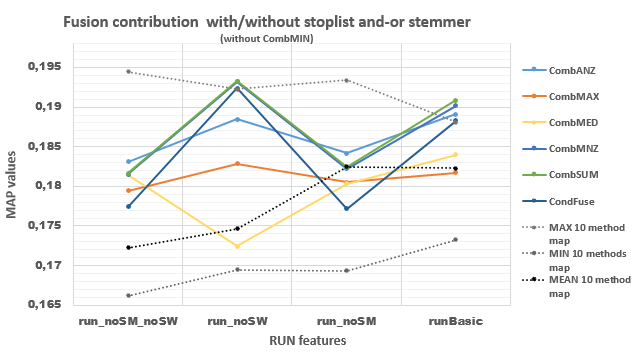
\includegraphics[width=\linewidth]{../eval/results-img-graphs/MAPFusSMSW.png}
			\caption{MAP for the fusions over different indexing and retrieval settings}				
			\label{fig:MAPFus}
		\end{minipage}
	\end{figure}

	The fusions' performances strongly depend on the input systems' performances. Both in the 10 models and in the fusions the best settings were achieved with the stemmer and with both stop list and stemmer.
	Adding the stop list to the stemmer doesn't change significantly the performance, and neither does using just the stop list compared to using an empty pipeline.
	This lead us to conclude that, in our collection and with the models selected, the stop list doesn't really affect the performance.
	
	Still, even though the fusions' performance may seem very similar to the models' one, the maximum and minimum MAP values are higher, and we noted a smaller variance between methods. 

	\subsubsection{Analysis on the performance's improvement using fusions}
	
	Finally, we focused on the improvement a fusion method can bring given a set of input models.
	
	Figures \ref{fig:MINincr}, \ref{fig:MEANincr} and \ref{fig:MAXincr} show how, over different retrieval and indexing settings, the fusion methods improve compared to the respective MIN, MEAN and MAX models' MAP.
	
	\begin{figure}	
		\begin{minipage}[H]{0.5\linewidth}
			\centering
			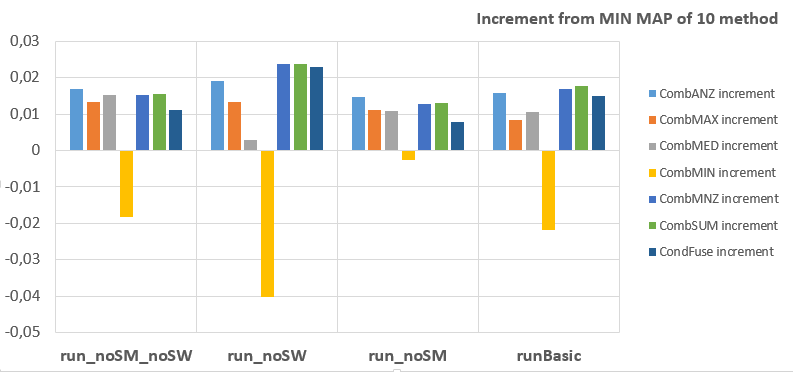
\includegraphics[width=\linewidth]{../eval/results-img-graphs/incrementFromMIN.png}
			\caption{Increment of the MIN MAP value compared to the MIN of the input models over different indexing and retrieval settings}				
			\label{fig:MINincr}
		\end{minipage}
		\begin{minipage}[H]{0.5\linewidth}
			\centering
			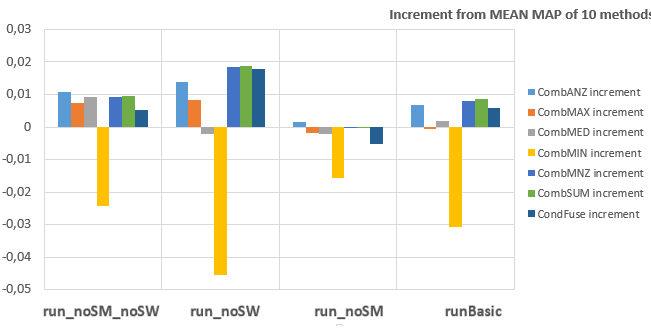
\includegraphics[width=\linewidth]{../eval/results-img-graphs/incrementFromMEAN.png}
			\caption{Increment of the MEAN MAP value compared to the MEAN of the input models over different indexing and retrieval settings}				
			\label{fig:MEANincr}
		\end{minipage}
		\begin{minipage}[H]{0.5\linewidth}
			\centering
			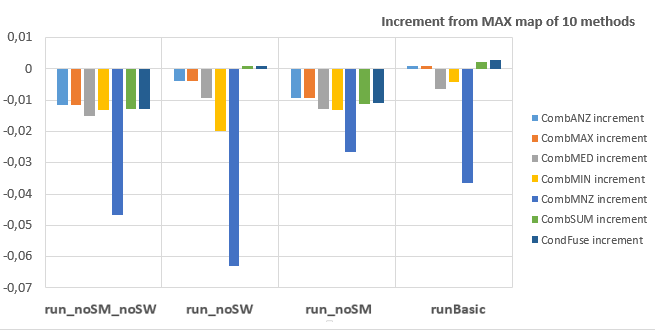
\includegraphics[width=\linewidth]{../eval/results-img-graphs/incrementFromMAX.png}
			\caption{Increment of the MAX MAP value compared to the MAX of the input models over different indexing and retrieval settings}				
			\label{fig:MAXincr}
		\end{minipage}
	\end{figure}
	
	These results show how there is always at least one fusion method that outperforms the ``basic'' models, even if the improvement is usually quite small.
	Condorcet ranks above the majority of fusion methods, bringing the biggest improvement when the input models are obtained with just the stemmer or with both the stemmer and the stop list.	
	
	\section{Conclusions}
	We implemented and tested different fusion methods. Our evaluation shows that, even if small, fusion methods actually improve the performance of the single models.
	
	But, the improvement isn't very big and it strongly depends on the performance of the input models, that is if the input models already have a good performance, the fusion will be better. Instead, the number of input system didn't affect the overall performances.
	
	Some fusion methods are clearly worse than others (like CombMIN), being always outperformed, while CondFuse is usually quite good, being one of the top fusion methods tested.

	\begin{thebibliography}{1}
		\bibitem{1}Lee, Joon Ho. ``Combining multiple evidence from different properties of weighting schemes.'' Proceedings of the 18th annual international ACM SIGIR conference on Research and development in information retrieval. ACM, 1995.
		\bibitem{2}Fox, Edward A., and Joseph A. Shaw. ``Combination of multiple searches.'' NIST special publication SP 243 (1994).
		\bibitem{3}Montague, Mark, and Javed A. Aslam. ``Condorcet fusion for improved retrieval.'' Proceedings of the eleventh international conference on Information and knowledge management. ACM, 2002.
		
	\end{thebibliography}
	

\end{document}
